\section{System Architecture}
\label{sec:architecture}

\subsection{Cache-Resident OS}

{\em CW: Promoted Cache Managment to its own section.
     May want to do the same for other subsections, and
     have the system architecture be a shorter overview,
     also serving as a roadmap for the reset of the paper.}

Entire OS stack remains resident in the processor cache.

\begin{itemize}
  \item Necessary kernel changes / gotchas
    \begin{itemize}
      \item Minimizing kernel size
        \begin{itemize}
          \item Removing unneeded drivers
          \item Memory allocator tweaks
          \item Example: {\tt struct page}
        \end{itemize}

      \item Boot order tweaks
        \begin{itemize}
          \item Two stage initrd
        \end{itemize}

      \item Never failing allocation
      \item Other shrinking memory footprint
    \end{itemize}
\end{itemize}

\subsection{Encrypted Main Memory}

\begin{itemize}
  \item Prior work
    \begin{itemize}
      \item TRESOR
      \item Cryptkeeper
      \item Various encrypted, authenticated, and oblivious RAM references
    \end{itemize}

  \item Keys kept in cache.
  \item Main memory used as an encrypted swap device
  \item AESNI
  \item Security assumptions
    \begin{itemize}
      \item confidentiality only
      \item XTS
    \end{itemize}
\end{itemize}

\subsection{Improved DMA Protections}

In order to be of practical use a software cryptoprocessor must allow use of I/O devices, such as those commonly used for storage and networking. These devices typically use DMA to move data between the device and main memory. In conventional operating systems memory for DMA operations is typically allocated from OS memory pools and may even reside on pages with other unrelated data. However, the combination of a cache-resident OS kernel and a security model where devices are treated as malicious brings up several issues that need to be addressed.

\subsubsection{Preventing DMA to cleartext data}
\label{sec:dma-prot}

In a software cryptoprocessor such as \vcage\, only the contents of the cache are in cleartext, while the rest of main memory is encrypted. In order to protect secrets and prevent modification of the system code and data, it is necessary to prevent any DMA operations to the portions of main memory that are cached. This can be achieved by employing DMA protection mechanisms such as Intel VT-d (IOMMU) Protected Memory Regions (PMRs), and Intel VT-d I/O Page Tables (xxx: refs?).

The protected memory regions consist of two pairs of base and bound registers; one only handles memory below 4GB while the other can address all of system memory. This provides considerably less flexibility than using I/O page tables. However, using I/O page tables requires at least a small number of pages from cacheable memory, which is a precious and limited resource. Placing the I/O page tables in uncached (untrusted) memory is not an option since the memory is treated as potentially malicious. In addition, the untrusted memory is marked as uncacheable to ensure it is not fetched into the processor cache, which has a negtive impact on the latency of memory accesses to the I/O page tables.

\subsubsection{DMA from untrusted memory}
\label{sec:dma-bounce}
Blocking DMA to cacheable memory regions protects the software cryptoprocessor and other cleartext data from being accessed by malicious devices. However, it means that we need to employ some form of bounce buffering (xxx: ref?) so devices are able to perform DMA using uncached memory. This is achieved by allocating a portion of the untrusted memory as a DMA bounce buffer. Unlike the rest of the uncached memory, the contents of this portion of memory are not automatically encrypted by the software cryptoprocessor. It may, however, contain encrypted data if the encryption has been performed by higher levels of the software stack \emph{e.g.} encrypted network traffic.

The Linux kernel provides a standard mechanism for hooking DMA operations by way of a global {\tt dma\_ops} variable which points to an instance of {\tt struct dma\_map\_ops}. We use this mechanism to provide our own set of DMA operations which copy data from system memory to the bounce buffer during {\tt map\_page}, {\tt alloc\_coherent}, or {\tt sync\_single\_for\_device} operations (xxx: mention ranger operations as well?), and vice-versa during {\tt unmap\_page}, {\tt free\_coherent}, or {\tt sync\_single\_for\_cpu} operations.

DMA bounce buffering provides the added benefit of preventing time-of-check time-of-use (TOCTOU) attacks. All untrusted data written by an I/O device is copied from the bounce buffer to kernel allocated I/O buffers which reside within the DMA protected region, before any data is made available to other software components. As a result, there is no race condition for a malicious device to exploit.

\begin{itemize}
  \item Wipe pages before DMA?
\end{itemize}

\subsubsection{Sub-page granularity}
\label{sec:dma-subpage}
Device drivers that allocate memory buffers for use during DMA often do so using the generic {\tt kmalloc} interface, which allocates memory from the size-specific slab caches. In the absence of any interception or modification of DMA transactions, it's possible for a device to access any kernel memory addressable by the DMA engine being used. Even with IOMMU protection and bounce buffering as outlined above, DMA buffers for multiple devices may end up being allocated from the same physical page, allowing a malicious or errant device to access data being read or written by another device.

In order to provide fine-grained partitioning between devices \vcage\ allocates DMA bounce buffers such that at any point in time the bounce buffer pages associated with different devices are disjoint. In practice this is achieved by allocating the entire page when either the start or end of the DMA buffer only uses some fraction of the page. While this increases the total amount of memory being used by the bounce buffer, since this is only done for \emph{in-flight} DMA operations, the overhead is manageable. (xxx: `manageable' sounds like a cop out)

\subsection{System Attestation}

\begin{figure}[h]
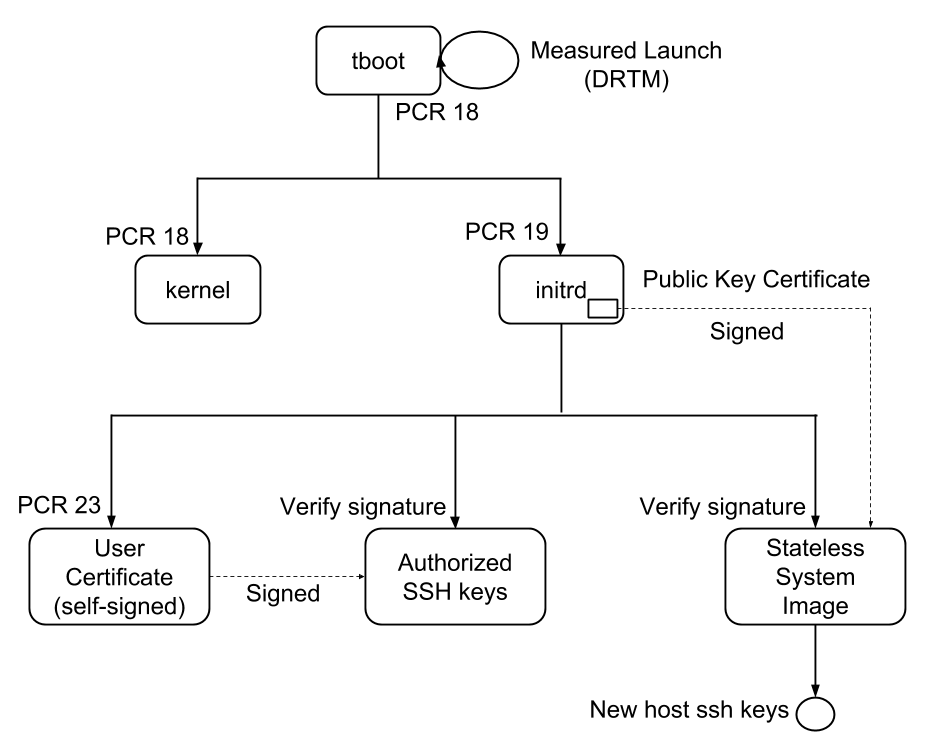
\includegraphics[width=\columnwidth]{drtm}
\centering
\caption{Root of Trust for vCage}
\label{fig-drtm}
\end{figure}

\begin{itemize}
  \item Trusted computing / TPM / TXT
  \item Chain of measurments
    \begin{itemize}
      \item tboot $\to$ kernel $\to$ initrd $\to$ keys
      \item PCR23
    \end{itemize}
  \item Stateless
  \item Keys regenerated on every boot
\end{itemize}

\subsection{System Hardening}
\label{sec:sys-hardening}
Built on a standard Linux kernel, the \vcage\ software cryptoprocessor utilizes various kernel level techniques to increase the security of the system, commonly referred as Linux Kernel Hardening \cite{SANS-hardening:2003}. In this section we describe those techniques in detail, and explain their role in increasing the overall resilience of the system to security threats.

\begin{itemize}
  \item Minimizing the attack surface: \vcage\ uses a minimized Linux kernel, containing a restricted set of system components and drivers. All interfaces to external devices and filesystems are minimal and carefully selected. In order to further close down any endangering communication ports, The only communication protocal that is allowed is SSH.
  \item Enforcing Linux security features: \vcage\ enforces Linux kernel security features including stack canary, Position Independent Executables (PIE), Data Execution Prevention (DEP) and Relocation Read-Only (RELRO) to protect against exploited structures in ELF binaries. Furthermore, it utilizes compilation-time security checks to detect potential string and buffer errors \cite{gcc-fortify}.
  \item Keeping a patched system: Security patches are regularly applied, and custom patches are created when a new vulnerability is disclosed.
  \item Grsecurity ready: Grsecurity is an extensive security enhancenment package to the Linux kernel \cite{Grsec}, incorporating numerous changes and touching nearly 2000 files. Some of its features include mitigation of common memory corruption exploits, Mandatory Access Control system and memory protections for userspace applications.
\end{itemize}
